\chapter{Alberi 2}

{Un albero è una particolare categoria di grafo}

\subsection{{[}NO{]}Definizione}

$G=(V,E)$ si dice albero {[}libero{]} se è aciclico e connesso.\\
Un albero libero in cui si seleziona un particolare vertice, chiamato ``radice'', si dice radicato.

{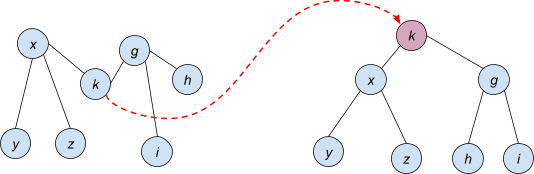
\includegraphics{images/image533.png}}

{Proprietà 1:}

Se $G$ è un albero, allora $\abs{E} = \abs{V} - 1$ poichè è, per definizione, connesso e aciclico:

\begin{itemize}
\tightlist
\item
  $G${~è connesso se $\abs{E} \geq \abs{V} - 1$ : si deve rispettare un numero minimo di archi}
\item
  $G${~è aciclico se $\abs{E} \leq \abs{V} - 1$ : si deve rispettare un numero massimo di archi}
\end{itemize}

{~~~~~~~~L'albero risulta essere quindi una struttura ``fragile'' per
quanto riguarda il numero di archi.}

{Proprietà degli alberi {[}liberi{]}}

{~~~~~~~~Sia }$G=(V,E) [NO]$ {, le seguenti affermazioni sono equivalenti:}

\begin{enumerate}
\tightlist
\item
  {$G$ è un albero}
\item
  {Due vertici qualsiasi di $G$ sono connessi da un unico cammino semplice, ovvero senza vertici ripetuti}
\end{enumerate}

{Dimostrazione:~~~~~~~~}

{Sia }$G=(V,E) [NO]$ {, per assurdo assumo ci siano almeno due vertici $u,v$, tali che esistono almeno due cammini che li collegano. Facendo ciò si forma un ciclo.}

\begin{enumerate}
\setcounter{enumi}{2}
\tightlist
\item
  $G${~è connesso, ma se un qualche
  arco viene rimosso da }$G${, il
  grafo risultante è disconnesso}
\item
  {$G$ è connesso e $\abs{E}=\abs{V}-1$}
\item
  {$G$ è aciclico e $\abs{E}=\abs{V}-1$}
\item
  {$G$ è aciclico, ma se un qualunque arco viene aggiunto, allora il grafo risultante è ciclico.}
\end{enumerate}

\subsection{Alberi di copertura}

{Un albero $G=(V,E) [NO]$ connesso si dice di copertura se tutti gli archi in $T \subseteq E$ toccano tutti i vertici di $G$.}

\subsubsection{Taglio di un albero}

{Un taglio di un albero è una divisione in due parti $(S,V\setminus S)$ dell'insieme dei vertici.}

{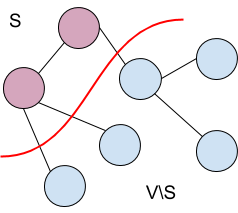
\includegraphics{images/image527.png}}

{Un taglio rispetta $A \subseteq E$ se non esistono archi di $A$ tagliati. Essi possono essere in una delle due partizioni ma non possono attraversare il taglio.}

\subsubsection{Arco leggero}

{Un arco è leggero se ha il peso minore tra gli altri archi attraversanti un taglio.}
